% Copyright (c) 2014,2016 Casper Ti. Vector
% Public domain.

\chapter{面向人工智能的云计算系统软件研究}
% \pkuthssffaq % 中文测试文字。
以深度学习为代表性技术的人工智能领域在21世纪10年代再度兴起,社会各界对于人工智能的需求也愈发旺盛。遍布超市和餐馆中的扫脸支付技术、智能手机上的语音智能助手、工厂中检测废件的自动检测装置等,都离不开人工智能技术的加持。具体的,上述场景都需要适当的机器学习模型在线部署以提供服务。

机器学习的工作流一般遵循如下几个步骤:1)模型开发与调试。在此阶段中,开发者根据具体的场景,编写并调试模型代码。2)模型参数调整。在这个步骤中,开发者使用训练集不断调整模型的超参数,使其在测试集上的表现符合某种标准(如准确率高于某个阈值)。3)模型部署,开发者将开发完成的模型部署到对应的场景中对外提供服务。

为了方便开发者专注到模型的开发流程中,各大主流云厂商均实现了支持机器学习模型开发-调试-部署整个流程的软件栈。同时,云厂商提供的一般性的平台可能无法满足用户特定的需求。因此针对具体场景,学术界也提出了一系列基于云服务的机器学习软件,以达到降低开发成本、提高模型在线服务的质量等目标。本章对上述内容涉及到的相关工作展开具体研究。

\section{一站式的云上机器学习系统}

本节先以AWS Sagemaker为代表,介绍公有云厂商一站式的云上机器学习系统。其它厂商中类似系统中对计算模型的抽象、使用方式等均与Sagemaker大同小异。

\subsection{AWS Sagemaker}\label{subsec_sagemaker}
AWS作为公有云领域的先驱者,在云计算的前沿技术领域一直处于领先的地位。其某些代表性技术甚至成为了多数公有云厂商所共识的标杆和规范。在机器学习系统这一分领域,其代表性系统为AWS Sagemaker。

Sagemaker是一个实现和产品化机器学习模型的框架\parencite{joshi2020amazon},用户可以将其模型训练需要的数据存储到AWS的对象存储服务S3中。然后,用户可以通过web的方式访问部署在云端的Jupyter Notebook服务,在线访问数据、编写并调试代码。当模型训练完毕后,可以使用Sagamaker内置的推理服务对模型进行发布。用户在发布时还可以根据平台的不同(云端或边缘节点)将模型打包编译成不同的版本。此外,Sagamaker还内置了一些常用的算法和数据集,方便开发者直接调用。

在训练算法和系统机制方面,Sagemaker旨在解决工业规模的模型训练场景中的如下几个常见问题:

\begin{itemize}
    \item \textbf{支持增量式的训练和模型更新。}在真实的工业场景中,几乎不存在完全静态的数据集。用来训练模型的数据集大多都是不断增长的。例如电商网站的用户行为数据,每天都在以相当的速度增长。在这样的动态数据上训练模型,势必要进行如下权衡:在全量数据上进行训练,可以获得质量更高的模型,然而时间和经济上的开销却会非常高;在最新更新的数据上(例如最近几天的数据)进行训练,可以快速的得到新的模型,却有可能在一定程度上牺牲模型的准确性。
    \item \textbf{容易估算训练模型产生的花销。}对于体量非常大的数据集,用户需要较为准确地估计训练模型将会产生的时间和经济花销。当今的云计算一般遵循按量付费的收费模式,因此云上的机器学习用户会格外关注花销的问题。
    \item \textbf{支持暂停和恢复模型训练,有一定的弹性。}生产环境中,大模型的训练通常包含跨越数十甚至上百台机器的并发任务。在一些场景中,由于超参数调整的需要或者计算资源的限制,开发者需要对这些任务进行中断和恢复。这就要求云上的ML系统能够支持大型训练任务中断和恢复时中间结果的保存和复原。
    \item \textbf{能够处理非持久性数据。}在很多场景中,数据并不一定是持久化的,也会有很多“瞬时”的数据,例如直播时的视频流等。这些数据一般不会被持久化保存,因此如何支持对这些数据的挖掘和学习也是一个重要的问题。
    \item \textbf{支持自动调参。}自动调参是一项非常耗时耗力的工作,特别是在生产环境的大数据集下。因此,如何能够支持高效的自动调参,方便用户选取合适的模型,对于云上的ML系统而言也是非常重要的。
\end{itemize}

下面将从计算模型、支持算法和具体的实现方式介绍Sagemaker如何解决上述问题。

\subsubsection{计算模型}
Sagemaker将机器学习训练的工作流抽象为三个阶段:initialize,update和finalize。initialize阶段:对相关的变量进行初始化。update阶段:系统以数据流及其状态作为输入,根据用户编写算法更新状态。在Sagemaker的后台,状态更新是在多台计算节点上同步执行的。finalize阶段:对之前所有的更新进行汇总,并输出最后的结果(对于机器学习任务而言,一般是一个模型)。通过上述抽象,用户只需编写initialize、update和finalize三个函数,就可以将整个训练过程交由Sagemaker,等待最后的模型输出。

算法~\ref{algo_sagemaker}用伪代码的形式讲述了三个阶段的具体流程。这里以计算一列数据的中位数为例,使用随机梯度下降(SGD)进行求解。对于如下一列数据:$x_1, x_2, x_3, ..., x_n$,则由如下公式给出这一列数据的中位数:$\operatorname{argmin}_z\Sigma_{i=1}^n||x_i-z||$。算法中的initialize函数首先对median和n两个参数做初始化。这里\textit{state}可以理解为一个key-value存储结构。在update阶段,函数将接收到的数据流\textit{data\_stream}分为若干mini\_batch,对每个batch没的数据,迭代式的对median值进行更新,同时更新n的值。最后,在finalize函数中,对最终的median值进行汇总。同时,系统还支持用户在算法的任意位置设置barrier(第15行),以对整个训练过程进行同步操作。

\begin{algorithm}
    \caption{Sagemaker计算模型}
    \label{algo_sagemaker}
    \begin{algorithmic}[1] 
        \Function{initialize}{$state$}
        \State $state.initialize('median', 0)$
        \State $state.initialize('n', 0)$
        \EndFunction
        \State
        \Function{update}{$state, data\_stream, synchronized$}
        \For {$mini\_batch \in data\_stream$}
        \State $current\_median \gets state.pull('median')$
        \State $n \gets state.pull('n')$
        \State $inc \gets 0$
        \State $batch\_size \gets 0$
        \For {$item \in mini\_batch$}
        \If {$item > current\_median$}
        \State $inc += 1$
        \Else
        \State $inc -= 1$
        \EndIf
        \EndFor
        \State $state.push('n', batch\_size)$
        \State $state.push('median',\frac{inc}{\sqrt{n + batch\_size}})$
        \If {$synchronized$}
        \State $state.barrier()$
        \EndIf
        \EndFor
        \EndFunction
        \State
        \Function{finalize}{$state$}
        \State \Return{$state.pull('median')$}
        \EndFunction
    \end{algorithmic}
\end{algorithm}

\subsubsection{支持算法}
尽管深度学习在近年越来越流行,特别是在学术界,各种刷新SOTA(即state-of-the-art,当前最优)效果的模型层出不穷。然而在产业界,经典的机器学习模型适用性依然非常广。本节对Sagemaker支持的广泛应用于产业界的经典机器学习模型做简单介绍。

\textbf{Linear Learner. }即线性回归模型,一般用来解决回归或者分类问题。在Sagemaker中,其支持使用随即梯度下降(SGD)来训练一个线性模型。特别地,Sagemaker还支持对一个模型指定不同的目标函数,并且并行地训练其对应的多个模型。

\textbf{Factorization Machines (FM). }FM常用于推荐系统中很多任务(例如CTR预估),是一种适用于分类和回归任务的更为通用的监督学习算法。FM是对线性模型的一种拓展,考虑了高维稀疏数据集中不同特征之间的关联。在Sagemaker中,FM也是通过SGD来进行训练的。

\textbf{K-Means Clustering. }K-Means聚类是一类无监督学习算法,可以将一个数据集聚为K个不同的类别。Sagemaker实现了一个流式计算版本的K-means,综合运用了来自随机优化、核心集和在线选址问题的思想。

\textbf{Principal Component Analysis (PCA). }即主成分分析,是一种通过尽可能保留数据集的方差来对数据进行降维的算法。Sagemaker实现了两种PCA算法。第一类是准确型的,通过适量的采样和特征提取,需要$O(d^2)$量级的内存大小。另一种是粗略型的,通过随即投影来减小内存开销到$O(kd)$。这里$k$和$d$分别代表主成分的个数和数据的维度。

\textbf{Neural Topic Models (NTM). }在Sagemaker中,NTM是一种用来在大型离散数据集中抽取latent representation的无监督学习算法,例如抽取文档中的语料库。为了实现更快的推理,NTM是基于variational autoencoder(VAE)模型实现的。

\textbf{Time Series Forecasting with DeepAR. }这是一种基于循环神经网络(RNN)的概率预测算法。和其它流行的时间序列预测算法不同,DeepAR使用一系列数据集训练了一个全局的模型,从而重点关注了在生产环境中常见的时间序列预测问题。

\subsubsection{实现方式}
经济和高效是云用户总是在关心的两类问题。Sagemaker为了满足这样的用户需求,充分利用了其底层的异构资源池,并通过上层的系统软件使得机器学习可以在成百上千台VM上横向拓展。

\textbf{在新硬件上运行ML任务。}
为了实现在异构的资源上(主要是CPU和GPU),Sagemaker中的大多数算法使用MXNet的库作为使用底层硬件的接口。MXNet通过一个张量算子构成的计算图来描述一个机器学习算法,同时通过将算子分配到具体的设备进行执行来实现并发地训练模型。

\begin{figure}[h]
    \centerline{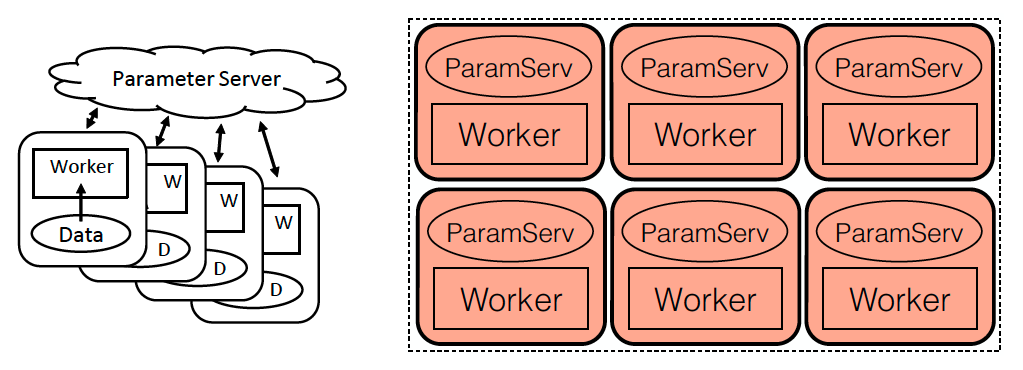
\includegraphics[width=\textwidth]{figures/ps-arch.png}}
    \caption{参数服务器系统架构。}
    \label{ps_arch}
\end{figure}

\textbf{利用参数服务器模型(Parameter-Server Model,即PS Model)实现分布式训练和参数共享。}如图~\ref{ps_arch}所示,在一个基于PS Model的集群中,服务器被分为两种,分别为worker和server。其中server负责保存模型所有需要训练的参数,worker负责具体的训练。在worker完成一轮迭代之后,会将更新后的参数变化量push到server端,并同步等待所有其它的worker完成此轮迭代。同步完成后,server汇总从worker端得到的变化量并对参数进行更新,而后worker再从server端pull更新后的参数,并继续进行下一轮迭代。值得一提的是,实际场景中为了追求训练速度,有时也会允许异步的参数更新,即不要求worker等待其它peer节点完成本轮计算,而是完成本地计算后就可以向server请求pull新的参数。这种弱一致性的设计会加快训练速度,通过也可能牺牲模型的质量。如图~\ref{sagemaker_ps}所示,在Sagemaker中,分布式训练就是通过参数服务器模型来实现的,且一般默认使用的是弱一致性的模式。同时,为了方便push和pull的操作,AWS实现了一个key-value的存储系统KVStore。

\begin{figure}[h]
    \centerline{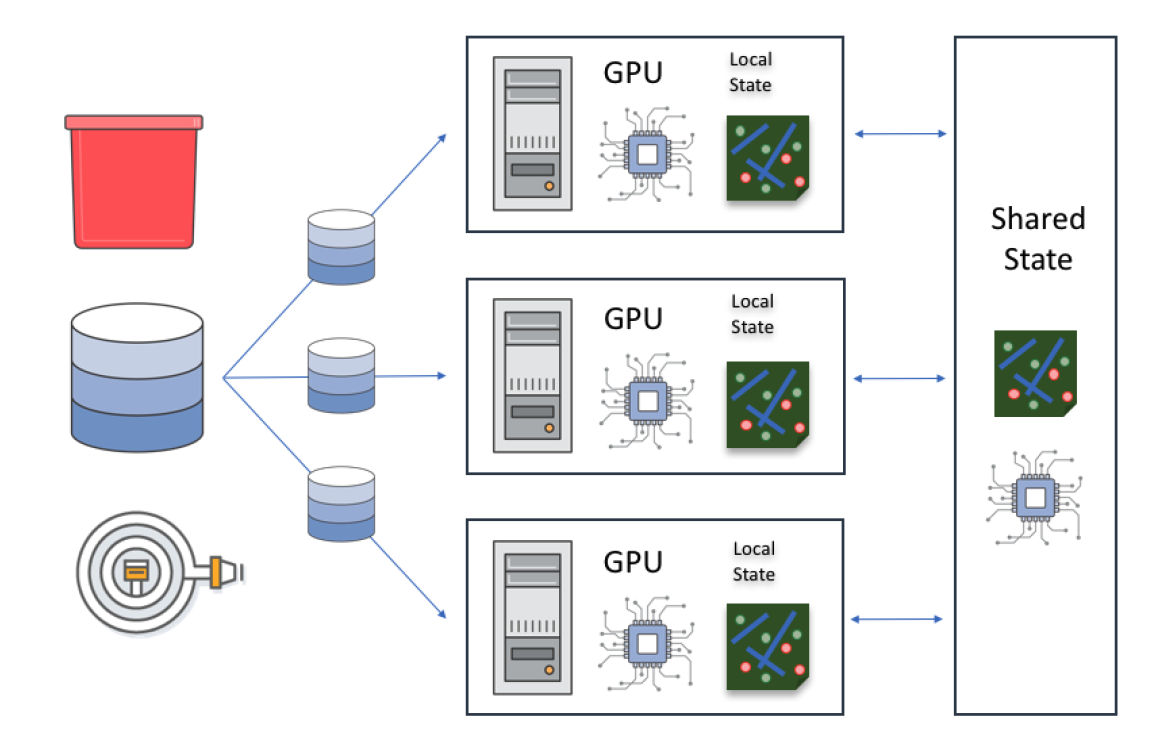
\includegraphics[width=\textwidth]{figures/sagemaker-ps.png}}
    \caption{基于PS Model的Sagemaker系统架构。}
    \label{sagemaker_ps}
\end{figure}

\textbf{模型抽象与参数表达。}Sagemaker在上层为用户提供了模型抽象和参数的表示方式。对于一个模型而言,有两个与其绑定的函数需要用户来实现:1)\textit{score}函数,为一个模型打分以衡量模型在该数据集的训练程度,在调试或者超参数调整阶段会被用到;2)\textit{evaluate}函数,接受一个batch的数据并计算该模型的输出。需要指明的是,对于不同的模型而言,输出的格式可能是不同的,例如对于分类问题,输出可能是一个label也可能是不同类别的概率。参数的表达方式同样需要统一的上层抽象。在Sagemaker中,不同类型的模型有着不同的表达形式。例如,K-means算法的模型就表现为一个核心集,因此,对于任意$k<k_{max}$,用户都无需重新训练模型,而是可以直接得到结果。对于K邻近算法,Sagemaker也有类似的设计。

\textbf{模型微调与超参数调整。}通常而言,一个超参数调整任务(Hyperparameter Tuning Optimization,即HPO)由多个并行的模型训练任务构成,这些训练任务每个都尝试一个不同的超参数组合,最后得到一个最优的配置。上述过程需要耗费大量计算资源和时间,对于寻常用户而言是非常耗时耗力的。而Sagemaker基于PS的计算模型设计保证了任意一个ML训练任务都可以随时启动和停止。这种机制使得模型微调和超参数调整变得更为容易操作:1)用户可以增量式地更新数据集,但却不用每次都重新训练模型,因为整个训练过程都是流式的;2)HPO可以同时启动多个训练任务,然后提前发现那些劣质的模型并将其终止,从而降低HPO的成本。

\subsection{其它厂商的相关系统}
总体而言,整个公有云环境中的机器学习系统都与Sagemaker大同小异,都使用了类似Parameter Server的分布式训练架构。例如阿里云的xxx,腾讯云的xxx。

\section{基于公有云服务的第三方机器学习系统}
尽管公有云厂商实现了相当完备的一站式机器学习系统,但是随着生产环境中业务场景的日渐复杂,大而全的公有云解决方案已经无法解决个性化的用户需求。例如,某些用户希望以尽可能低的成本完成大型模型的训练,或者在保证模型服务的SLO前提下,能够尽可能低成本的部署机器学习模型。在上述场景中,为了完成用户的具体需求,需要综合利用各类云资源,并制定一定的策略。本节对近几年来几个构建于公有云资源上层的机器学习系统做具体介绍。
\subsection{基于云厂商动态资源的机器学习模型训练系统}
% Proteus by harlap
% SpotTune by Yan
机器学习模型的训练是一个不断在给定数据集上迭代更新参数的过程。对于一些较大的模型,训练时间一般会非常长。特别是深度神经网络模型再度兴起后,模型开始变得越来越庞大。例如Open AI的自然语言模型GPT-3,包含1750亿个参数,单单存储这些参数就需要450GB的空间。而训练该模型的成本,据估计更是达到了1200万美元。对于一些个人开发者和小型公司,大模型的训练往往显得遥不可及。

除了上述可训练的参数之外,还存在大量不可训练的参数。例如,SVM模型中核函数的类型,树模型中树的深度,深度神经网络模型中网络的宽度和深度等。这些参数需要由开发者在训练之前事先决定,一般被称为超参数。不同的参数组合在一起,就构成了巨大的搜索空间。例如,如果存在6个超参数,每个超参数有4种不同的选择,就会产生$4^6=4096$种不同的超参数组合。

完全遍历所有的超参数组合是非常费时费力的,通常情况下也是不切实际的。研究者为了减少超参数搜索的此时,提出了诸如网格搜索、贝叶斯搜索等技术。但即便如此,仍然需要大量的算力来支撑整个搜索过程。

而与此同时,在云计算时代,云上资源的易用性、高度的弹性以及收费模式的多样性使得以较低的成本完成费时费力的模型训练和超参数搜索变为可能。如上一小节所述,一些云厂商提供了一些价格低廉的动态资源。和一般的可以获得可用性保障的资源相比,这类资源拥有相同的计算能力,但是可用性比较低,在某些场合会被云厂商主动回收。基于上述事实,可以形成一个直观的想法:在这类廉价的资源上运行机器学习模型训练和调参任务,并辅以一定的容错策略和资源选择策略,可以显著降低成本。

\begin{figure}[h]
    \centerline{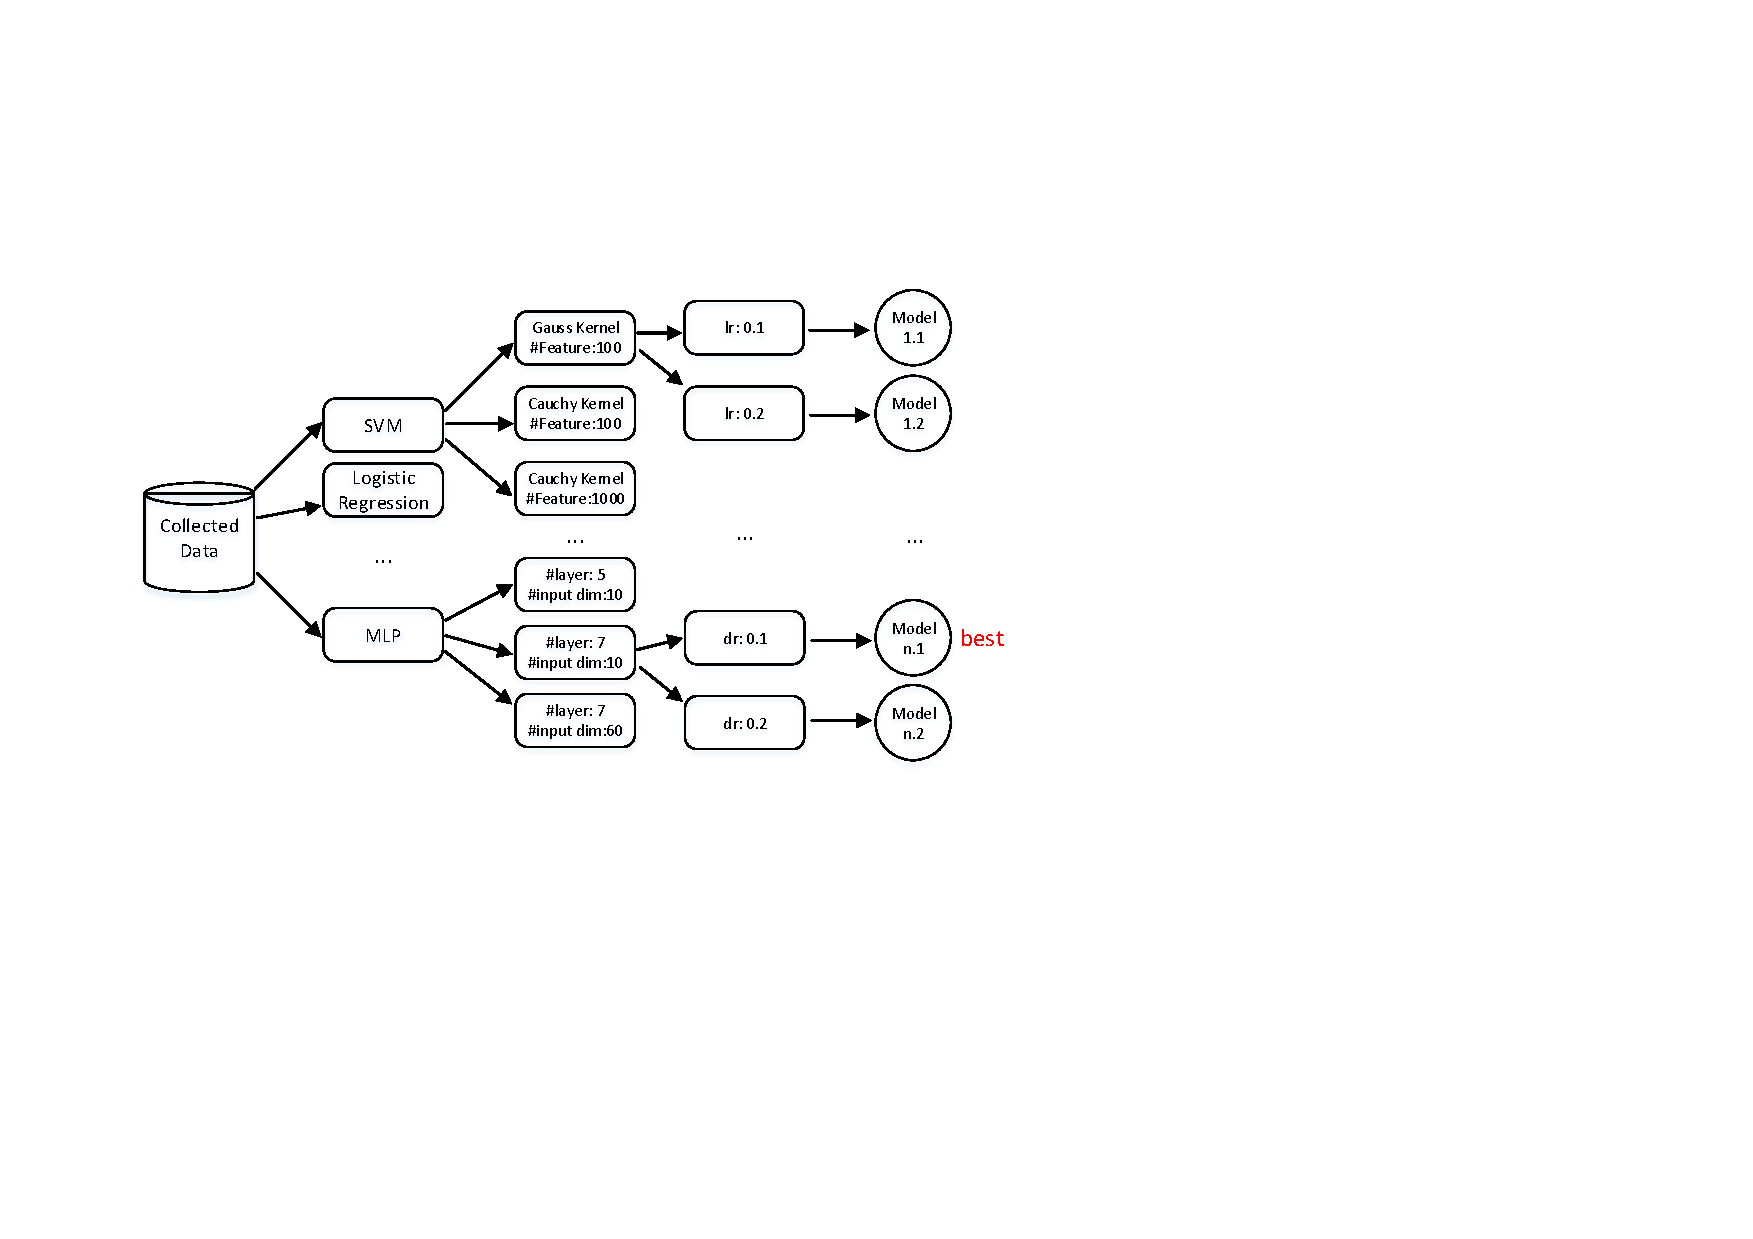
\includegraphics[width=\textwidth]{figures/hpt.pdf}}
    \caption{一个超参数调整的例子。}
    \label{hpt_example}
\end{figure}

但是,在动态资源上运行机器学习模型训练和调参,虽然直觉上会降低成本,但是可能会产生额外的风险。因此,要做到高效并可靠地在动态资源上运行上述作业,还有如下若干问题需要解决:

\textbf{1. 及时处理中断。}动态资源之所以廉价,是因为其稳定性比较低。通常情况下,在某些特殊情况下(例如集群中的负载比较高,需要动态资源来补充资源池),云厂商有权利主动回收这些动态资源。如果不处理这种回收引起的中断,机器学习模型的训练就要被动终止。因此需要采取一些手段,例如提前保存模型或者迁移任务,以及时处理中断。

\textbf{2. 合理的资源选取算法。}事实上,这是在云上运行任务时需要考虑的一个通用问题。用户在云上运行作业时,一般会有一个目标,例如作业运行时间最短或者最终的总体成本最低。因此需要通过一定的算法,为用户选取能满足其需求的资源。对于机器学习模型训练与调参任务亦是如此。

\textbf{3. 充分利用云的弹性。}事实上,在机器学习模型训练过程中,存在大量的无效计算。如图~\ref{hpt_example}所示,经过大量的参数尝试,最终只剩余一个有效模型(即效果最好的模型)。因此,在参数搜索的过程中,大量的计算是无效计算。而云计算的一个重要特点就是高弹性,即用户可以因为负载增加随时获取资源,也可以因为资源闲置随时释放资源。如果效果不好的模型能够被提前发现,并释放掉其占用的计算资源,则可以避免大量无效计算,从而进一步节省成本。

\textbf{4. 对计算框架进行定制。}现有的流行的机器学习框架如Tensorflow,PyTorch,MXnet等,一般都假设底层的计算资源是可靠的,因此都没有针对上述动态资源进行适配。如果要在动态资源上运行ML任务,则需要对框架进行深度定制,使其具备一定的容错能力。

为了解决上述问题,使ML模型训练和调参都可以在云上经济高效地进行,许多研究者提出了若干解决方案。A. Harlap等人在2017年提出了ML模型训练系统Proteus\parencite{harlap2017proteus},针对Parameter Server架构的ML模型训练框架对AWS和Google Cloud的动态资源做了适配,使其能高效经济地在之上运行;Y. Li等人在2020年提出了SpotTune\parencite{li2020spottune},将ML调参任务部署在AWS动态资源上,并结合一定的资源选取算法和训练趋势预测算法,使调参任务节省大量的无效计算,最终达到了经济高效的目的。下文对较有代表性的Proteus和SpotTune做较为详细的介绍。

在介绍相关系统之前,有必要对目前云市场上常见的资源类型、本节重点研究的动态资源及其收费模式做简要介绍。

云计算作为互联网时代下的一种新型计算模式,通过虚拟化和软件定义技术将服务器、存储、网络甚至软件等各种资源聚集为共享资源池。这些虚拟资源用则进行分配,而且种类和数量均可按需配置并按实际用量计费,不用则回收到资源池中等待下次分配。相比传统的IT 资源使用模式,云计算这种按需使用、按量付费的特点增加了用户的灵活性,但也导致了用户需求的不确定性。比如:在销售旺季,用户使用云的频率就会增加,云服务商的负载压力会持续增大甚至超过峰值,进而可能导致故障;而在销售淡季,用户使用云的频率就会大幅下降,云服务商的负荷压力也会大幅降低,导致了空闲资源的浪费。为了充分利用云资源池中的空闲资源,云服务商推出了多种的计费模式,试图以多样化的价格来吸引用户的同时,确保自己在需求高峰时可以回收部分资源。

\begin{table}[!htbp]
    \caption{亚马逊公有云EC2计费模式分析}
    \centering
    \label{tbl_inst_types}
    \begin{tabular}{|c|c|c|c|}
    \hline
    \diagbox{计费模型}{比较}&计费公式&计费特点&适用场景\\
    \hline
    按需实例&\tabincell{c}{实例运行时\\长*单位时\\间对应实例\\费率}&\tabincell{c}{单位时间费率固定,\\无需用户有任何使用\\承诺,价格较高}&\tabincell{c}{适合使用需求周期较\\短、对实例运行环境\\需求多变的用户}\\
    \hline
    预留实例&\tabincell{c}{签约金+$\Sigma$\\第i次运行时\\间*单位时\\间费率}&\tabincell{c}{用户与亚马逊签订长\\时间使用合约,并交\\付签约金,在“合同”\\期内使用EC2 需额外\\支付费用,但费率适\\中}&\tabincell{c}{适合使用需求周期长\\且实例对运行环境性\\能要求稳定的用户}\\
    \hline
    竞价实例&\tabincell{c}{实例运行时\\长*单位时\\间对应实例\\费率}&\tabincell{c}{单位时间实例费率变\\动,根据实例的需求\\情况以拍卖的方式决\\定,费用较低}&\tabincell{c}{适用于没有即时性要\\求、任务可中断的业\\务}\\
    \hline
    \end{tabular}
\end{table}

以亚马逊公有云为例,如表~\ref{tbl_inst_types}所示,EC2 按照计费模式可划分为按需实例(Ondemand Instance)、保留实例(Reserved Instance)和竞价实例(Spot Instance)这三类。相比较于按需实例和保留实例,竞价实例可提供超低折扣,但其价格会随着供需关系而不断调整。用户需要为获取该实例设置一个最高的出价,如果当前市场的价格低于用户的出价,则用户获得实例资源进行计算。一旦市场价格高出用户的出价,则该计算资源会被亚马逊收回。对于公有云厂商来说,竞价实例通过市场机制发掘了云资源的真正价格,达到了其尽可能以最合理的价格卖出最多闲置资源的目标。而对于云平台上的虚拟云用户来说,各种无状态、或者具有容错能力的应用程序可以基于竞价实例来大幅度降低运行成本,代表负载包括:大数据、容器化工作负载、CI/CD、Web 服务器、高性能计算(HPC) 以及其它测试和开发工作负载。尽管竞价实例的出现为非在线业务或者成本敏感业务提供了一种全新的计算资源类型,但是目前来看,无论用户的业务类型为哪种,大部分用户选择的资源依旧是为在线业务所准备的按需实例和保留实例。

竞价实例与按需实例、保留实例的合理使用,可以帮助虚拟云用户优化工作负载的成本和性能。根据AWS 官方博客,已经有不少大型企业(如本田汽车)成功使用AWS 的竞价实例把部分业务的计算成本下降高达70\% 。然而有效的使用竞价实例除了对负载自身的要求以外(如可中断等),还需要用户针对自身的应用场景选择“正确”的实例类型。由于竞价实例在价格和回收方面的不确定性,这是比较复杂的。

Proteus是一个基于Parameter-Server(下文简称为PS)架构的机器学习系统。PS是大规模机器学习系统中常用的架构,其系统架构在\ref{subsec_sagemaker}中已描述。如其文中描述,其使用了敏捷的弹性机制并辅以“激进的”竞价策略,使得机器学习任务在云上高效经济地完成。Proteus由两个主要组件构成:AgileML和BidBrain。

其中,AgileML是负责协调整个PS架构的主要组件。其通过如下的基本思想,在保证整个系统可用性的前提下,尽可能多使用动态资源(即AWS Spot Instances)以降低成本:1)将PS的关键功能节点(即保存模型参数的server节点)部署在可靠资源上(如AWS的按需实例或者预留实例);2)将PS的worker节点(即负责实际计算和参数更新的节点)部署在动态资源;3)当动态资源和可靠资源的比例不同时,AgileML会采取不同的策略。具体地,当比例比较小时(例如2:1),其简单地将server节点分布在所有的可靠资源上,而当比例比较大的时候(例如63:1),其将可靠资源作为BackupPSs而将动态资源作为ActivePSs,当发生参数更新时,更新会先到达ActivePSs。同时,在网络带宽允许的前提下,ActivePSs上会启动相应的后台任务将参数同步到BackupPSs上。

BidBrain是Proteus中的资源管理模块,决定何时获取和释放动态资源。据文中所描述,BidBrain是专为AWS EC2定制的,但是其经过少量的修改和定制化也可以适用于其它环境(如私有集群和其它公有云市场)。其秩序性地监控云市场中动态资源的价格,并即时地竞标那些可能给当前计算带来增益的资源(文中通过 work per dollar来衡量增益,即单位花费可以完成的工作量)。类似地,当一种资源在达到其第一个小时的末端时,就有可能因为性价比降低而被释放掉。另外BidBrain还利用了AWS EC2的一项特殊规则:当资源在其第一个小时内被释放时,其所有花费会被退回。因此其也会主动获取那些在接下来的一小时内会被释放掉的资源,以进一步降低整个成本,此种策略被作者成为激进的竞标策略。总体而言,BidBrain会在激进的竞标策略和保守策略之间权衡,以寻求整个系统的收益最大化。



\subsection{基于FaaS的模型训练系统}
%infocom 19

\subsection{基于公有云服务的模型部署系统}
% MArk
% Tributary

\subsection{基于FaaS的模型部署系统}
%一系列FaaS for ML serving的工作,INFaaS etc

\section{小结}
% vim:ts=4:sw=4
